\chapter{蓄電池を用いた高速化手法}
\label{chap:proposal}

前章でデータセンタにおける電力コスト削減要請についての背景および関連研究を紹介した。実は電力削減はデータセンタだけに限らず、コンピュータアーキテクチャ全体の共通の課題である。その中でもHPC(High Perfomance Computing)領域においては消費される電力は物理的制約による供給可能電力に達しつつあり、近い将来スーパーコンピュータの性能は電力供給能力によって頭打ちになると予想されている。そのため与えられた電力制約下において性能の高いシステムの構築が必要とされている。本章ではその実現手法のひとつとして、既存設備に含まれる蓄電池を用いた電力制約下での性能向上手法を提案する。


\section{フェーズ間の電力融通手法の提案}
\label{sec:curb}

\begin{figure}[t]
 \begin{center}
  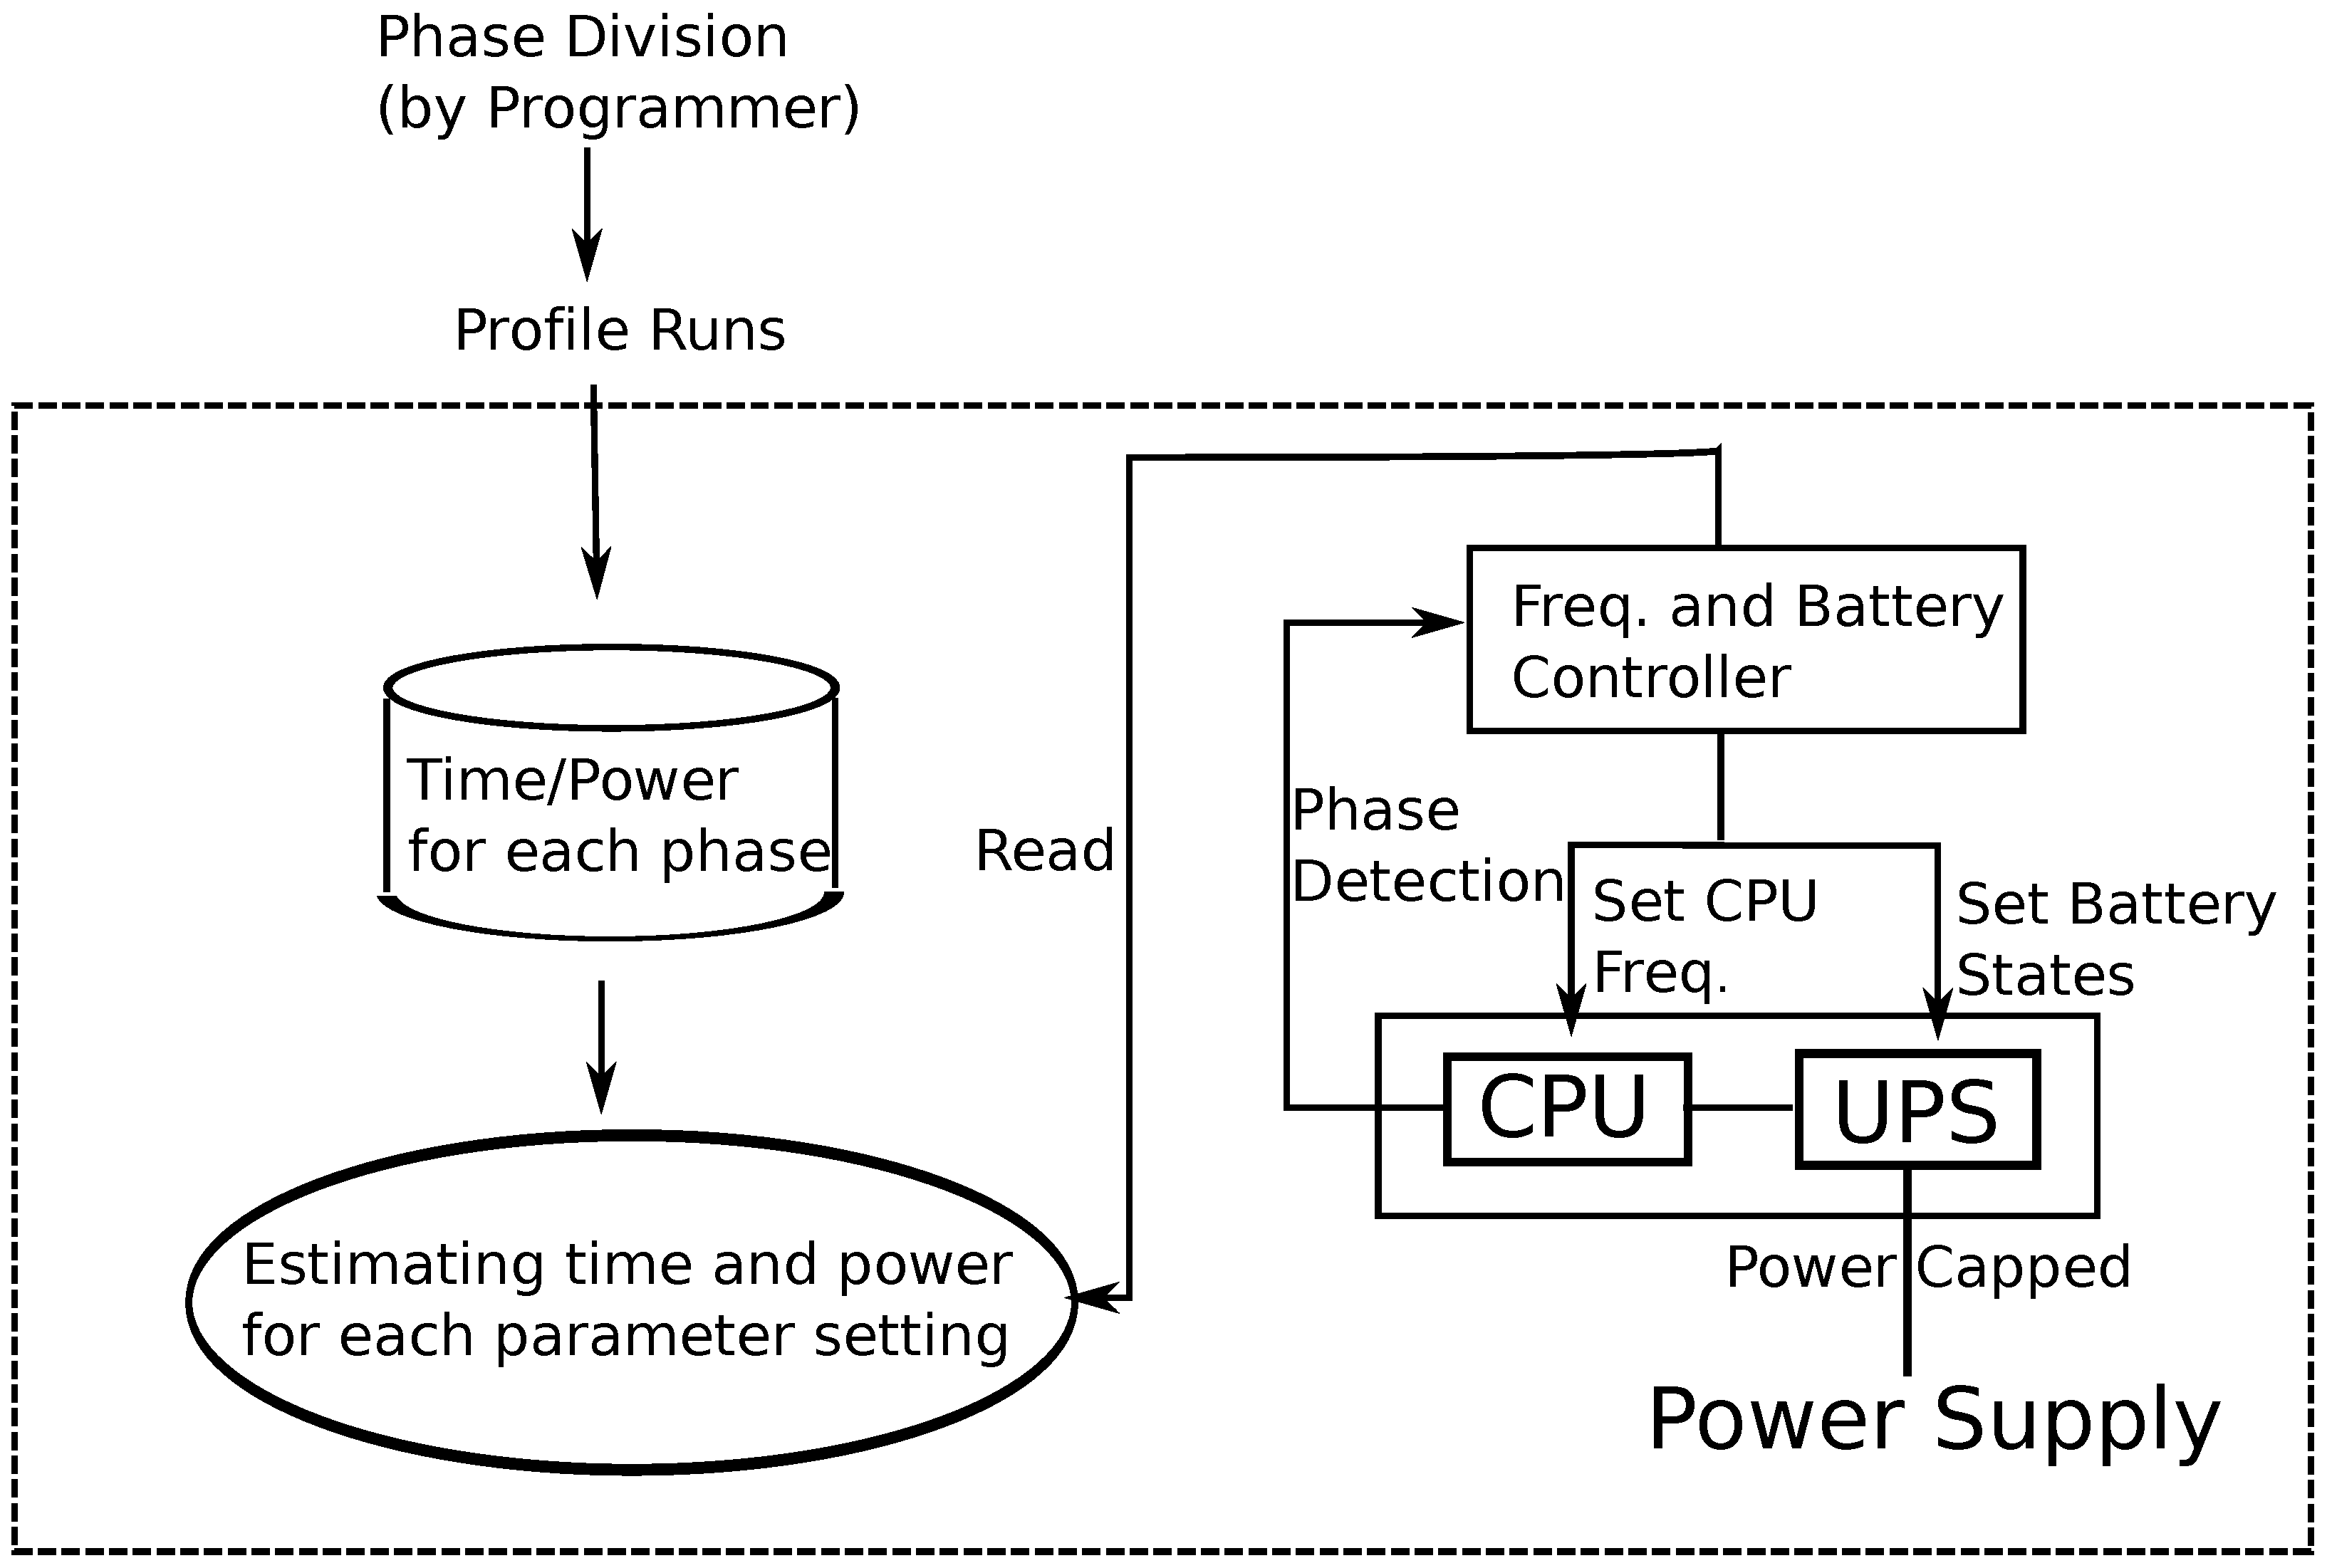
\includegraphics[width=110mm]{proposal_overview.eps}
 \end{center}
 \caption{提案手法の全体像}
 \label{fig:proposal_overview}
\end{figure}

図\ref{fig:proposal_overview}に提案手法の全体像を示す。提案手法では、まずプログラマが\ref{sec:phase2}節で述べる、フェーズの開始と終了を示す文をアプリケーションのソースコードに埋め込む。次に、プロセッサが取りうる全ての周波数を設定し、アプリケーションのテスト実行を行う。このとき、提案システムはプログラマによって埋め込まれたフェーズ区切り文を読み取り、各フェーズでの平均電力・実行時間を計測し、プロファイル情報を作成する。プロファイル情報をもとに、提案システムは\ref{sec:algorithm}節で述べるアルゴリズムを用いて最適な充放電計画を決定する。最適な充放電計画とは、与えられた電力制約下において実行時間を最小とするような、フェーズごとのプロセッサ周波数及び充放電量である。本番実行時にはそれぞれのフェーズが実行される直前に、提案システムによって前述した充放電計画に従ってプロセッサの周波数が設定されることにより、最適な充放電制御が行われることになる。ここで、プログラマが行わなければならない作業はソースコードにフェーズ区切り文を埋め込むことのみであり、最適な充放電計画の決定及び実行は提案システムによって自動的に行われることに注意されたい。

\subsection{蓄電池を用いた電力融通によって実現される\\実行時間短縮のメカニズム}

スーパーコンピュータ上で走るアプリケーションは実行時間が長く、実行が進むにつれて処理の特性が大きく変化するものも多い。CPUによる演算中心の処理やメモリアクセスなどのI/Oが中心の処理、プロセス間の通信が中心の処理など、異なる処理は基本的に異なる特性を持っている。また同じ処理であっても演算の並列度などの他の多くの要因に処理の特性は影響される。一般に処理の特性が異なると、その処理にかける電力と処理を終えるまでの実行時間の関係を表した電力−実行時間曲線は異なったものになる。

本手法では処理の特性の違いによる電力−実行時間曲線の違いに着目する。アプリケーションの中に異なる電力−実行時間曲線をもつ区間(以下、それぞれの区間をフェーズと呼ぶ。)が複数ある場合には蓄電池を用いた電力融通を行うことで、以下の3つの効果により電力制約下での性能向上を行うことができると考える。

\begin{description}
\item[ケース1] \mbox{} \\電力を増やしたときに実行時間があまり短縮されないフェーズから実行時間が大きく短縮されるフェーズへと電力融通を行うことによる性能向上
\item[ケース2] \mbox{} \\電力消費が小さく、電力制約分の電力を使い切れないフェーズで生じた余剰電力を他のフェーズへ融通することによる性能向上
\item[ケース3] \mbox{} \\周波数が離散的であるために生じる余剰電力を融通することによる性能向上
\end{description}


まず、ケース1の効果について説明する。異なる電力−実行時間曲線において、かける電力を変化させたときの実行時間の変動の大きさは異なる(図\ref{fig:power_time_proposal})。かける電力を減らしても実行時間があまり短くならないフェーズから、電力を多くかけると実行時間が大きく短くなるフェーズへ蓄電池を用いて時間方向へ電力を融通することにより実行時間を短縮することができる。

\begin{figure}[t]
 \begin{center}
  \includegraphics[width=110mm]{power_time_proposal.png}
 \end{center}
 \caption{電力−実行時間曲線の違いによって、かける電力の増加による短縮される実行時間が異なる様子(ケース1の効果)}
 \label{fig:power_time_proposal}
\end{figure}

次に、ケース2の効果について説明する。軽い処理を行っているフェーズでは、プロセッサを最大周波数で動かしても電力制約分の電力を使い切ることができない。従来ではその余剰電力は無駄になっていたが、蓄電池を用いれば電力制約以上の電力を必要としている他のフェーズへその電力を融通することができ、性能向上が見込める。\ref{sec:capping}節で紹介したデータセンタにおける蓄電池を活用した電力融通手法では、この効果により電力ピークカットを実現している。

最後にケース3の効果についてであるが、現在のプロセッサは離散的な有限の数の周波数でしか動作することはできない。そのため、電力制約によって最高周波数で動作できない場合であっても、使い切れていない電力というものが存在する。例えば、消費電力80Wおよび60Wの2種類の動作周波数をサポートしているプロセッサに対して70Wの電力制約をかけた場合、プロセッサは消費電力60Wの周波数でしか動作することができないので、10Wの電力を使い切れないことになる。蓄電池を用いればこの余った電力も他のフェーズへ融通することができるので、その分実行時間の短縮に繋がると考えられる。

以上の3つの効果による電力制約下での性能向上が本論文の提案手法である。次節以降では、アプリケーションの区切り方および電力融通をどう行うかについての各論を述べる。


\section{フェーズの要件}
\label{sec:phase1}

\ref{sec:curb}節で述べたように、本手法では処理ごとの電力−実行時間曲線の違いを利用して性能を向上させる。そのため、電力−実行時間曲線の異なる区間をそれぞれ別のフェーズとして定義する。フェーズの区切り方が細かいほど電力融通の機会は増えることになるので、理想的なバッテリーを用いる場合には、アプリケーション内の電力−実行時間曲線が異なる区間全てを別のフェーズとして区切る場合が理想的なフェーズの区切り方となる。

しかし、実際のバッテリーはあまり高頻度に充放電を行えない・充放電の速度に限界があるなど様々な物理的制約がある。また、フェーズの数が多くなるほど\ref{sec:formularization}節で述べる電力融通問題を解くことが困難になる。さらに、入力データが異なる場合には処理の順序が異なるので、どの時刻にどの処理が行われているかが分かりにくく、アプリケーション内の電力−実行時間曲線が異なる部分を全て求めること自体も難しい問題である。そのため、現実の問題を扱う場合には電力−実行時間曲線が異なる全ての部分ではなく、もっと粗い粒度でフェーズを区切ることになる。

\section{フェーズの求め方}
\label{sec:phase2}

HPC領域において、アプリケーションの性質や演算装置の特徴に応じてソースコードに手を加えることは珍しいことではない。ソースコードに手を加えるときに手間となるのはソースコードを書き直すことである。以下のコードはCPU並列化プラットフォームのOpenMPのコードであるが、このようにいくらかのコードを書き足す程度であればプログラマの大きな負担にはならない。

{\small
\begin{itembox}[c]{OpenMPのソースコード}
\begin{verbatim}
int main(int argc, char *argv[])
{
    int i;
#pragma omp parallel for       //性能向上のために追加される唯一の行
    for(i = 0; i <= 10000; i++)
    {
        // (並列処理させたいプログラム)
    }
}
\end{verbatim}
\end{itembox}}

本手法では、上の例のようにユーザプログラマにいくらかのコードを足してもらうことによりフェーズを区切る。具体的には以下のようになる。

{\small
\begin{itembox}[c]{本手法で想定するフェーズの指定方法}
\begin{verbatim}
int main(int argc, char *argv[])
{
#pragma phase start A    //フェーズAの始まりを示す
    //フェーズAの処理
#pragma phase end A      //フェーズAの終わりを示す
    //何らかの処理(ない場合もある)
#pragma phase start B    //フェーズBの始まりを示す
    //フェーズBの処理
#pragma phase end B      //フェーズBの終わりを示す
}
\end{verbatim}
\end{itembox}}

この区切りを示すコードは、時系列的に異なる処理の部分に配置さえされていれば、以下のように繰り返し文の中に入っていたり、他の関数にまたがっていたりしても構わない。

{\small
\begin{itembox}[c]{繰り返し文における例}
\begin{verbatim}
int main(int argc, char *argv[])
{
for(i = 0; i <= 10000; i++)
{
    #pragma phase start A    //フェーズAの始まりを示す
        //フェーズAの処理
    #pragma phase end A      //フェーズAの終わりを示す
    #pragma phase start B    //フェーズBの始まりを示す
        //フェーズBの処理
    #pragma phase end B      //フェーズBの終わりを示す
    }
}
\end{verbatim}
\end{itembox}}

{\small
\begin{itembox}[c]{関数にまたがっている場合の例}
\begin{verbatim}
functionA()
{
#pragma phase start A    //フェーズAの始まりを示す
    //フェーズAの処理
#pragma phase end A      //フェーズAの終わりを示す
}

functionB()
{
#pragma phase start B    //フェーズBの始まりを示す
    //フェーズBの処理
#pragma phase end B      //フェーズBの終わりを示す
}

int main(int argc, char *argv[])
{
    functionA();
    functionB();
}
\end{verbatim}
\end{itembox}}


\section{電力融通問題の定式化}
\label{sec:formularization}

\ref{sec:phase2}節の手法によってアプリケーションが$n$個のフェーズに区切られていて、それぞれのフェーズが1から$n$までの番号を一意に割り振られている状況を考える。フェーズ$i$(ただし$1\leq i\leq n$)における電力−実行時間曲線を$T_i(p)$と定義する。$T_i(p)$はフェーズ$i$にかける電力$p$に対して、フェーズ$i$を終えるのにかかる実行時間を返す関数である。$T_i(p)$はフェーズ分割が行われていれば、それぞれのDVFSパターンについてテスト実行を行うことで得ることができる。この点については\ref{sec:method}節で詳しく述べる。

本論文での目的は、与えられた電力制約下においてアプリケーション全体の実行時間を最小化することである。そこで、与えられる電力制約を$p_{max}$とする。そして本手法ではフェーズごとに蓄電池を用いて電力を融通するため、フェーズ$i$において蓄電池から供給される電力を$\Delta p_i$とする。$\Delta p_i$はマイナスのときは蓄電池に充電することを意味する。

以上の変数を用いて最適化問題として定式化すると、以下のようになる。

\begin{eqnarray}
{\rm min } & \sum_{i=1}^n T_i(p_{max} + \Delta p_i) \label{asm:min} \\
{\rm s.t. } & \sum_{i=1}^n \Delta p_i T_i(p_{max} + \Delta p_i) \leq 0 \label{asm:s.t.}
\end{eqnarray}

式(\ref{asm:min})は実行時間の最小化を意味する。式(\ref{asm:s.t.})の左辺は、アプリーケション実行の全体を通して、蓄電池から供給されるエネルギを意味している。蓄電池はあくまで電力を時間方向に融通しているだけであり、エネルギを増やすことはできない。そのため、式(\ref{asm:s.t.})はエネルギ保存制約式となる。

また、$T_i(p)$はおおまかに近似をとると式(\ref{asm:model})で表される直角双曲線になるため、式(\ref{asm:min})、(\ref{asm:s.t.})で定式化される最適化問題は非線形計画問題となる。

\begin{eqnarray}
T(p) = a_0 + \frac{a_1}{p-a_2} \label{asm:model}
\end{eqnarray}

ただし、ここで対象としている蓄電池は以下のような特徴をもつ理想的な蓄電池である。

\begin{enumerate}
\item 電池容量無限
\item 充放電速度無限
\item 充放電によるエネルギ損失はない
\end{enumerate}

想定している蓄電池では電池容量が無限であるので、アプリケーションの実行前後でのエネルギが保存されていれば、アプリケーションの実行途中で電池容量がゼロになることはない。同様に、充放電速度が無限でエネルギ損失はないので、充放電することにより失われる電力はゼロである。


\section{電力融通問題の解法}
\label{sec:algorithm}

非線形計画問題を解くアルゴリズムはいくつも研究されている。しかし、\ref{sec:curb}節でも述べたように現実のプロセッサは有限の数の周波数でしか動作することはできない。そのため、式(\ref{asm:min})、(\ref{asm:s.t.})の中の$\Delta p_i$は有限のパターンしか存在しない。本論文では$\Delta p_i$が有限個の値しか取れないことを利用して、全てのフェーズにおいて取りうる全ての$\Delta p_i$を実際に代入してアプリケーション全体の実行時間を計算することにより、最適な$\Delta p_i(1 \leq i \leq n)$を求める。また、フェーズ$i$での充放電量$\Delta p_i$と動作周波数$f_i$は1対1に対応づけられるので、それぞれのフェーズにおける動作周波数$f_i(1 \leq i \leq n)$も求められることになる。






